\section{Введение}

Многие задачи в науке и технике включают многократное решение сложных систем дифференциальных уравнений в частных производных (PDE) для различных значений параметров. Примеры возникают в молекулярной динамике, микромеханике и турбулентных потоках. В данной главе рассмотрен метод нейронного оператора Фурье.

\section{Литература}

	\begin{itemize}
		\item ~\cite{FNO} --  работа, в которой описан подход нейронного Фурье оператора для  дифференциальных уравнений в частных производных
		\item ~\cite{Deeponet} -- работа, в которой описан подход нейронного оператора. На основе данной статьи построен метод нейронного Фурье оператора
		\item ~\cite{FNOcode} -- код с реализацией метода нейронного Фурье оператора 
	\end{itemize}


\section{Нейронный Фурье оператор для дифференциальных уравнений в частных производных}

Традиционные методы, такие как методы конечных элементов (FEM) и методы конечных разностей (FDM), решают уравнения путем дискретизации пространства. Грубые сетки работают быстро, но менее точно; подробные сетки точны, но медленны. Сложные системы PDE обычно требуют очень точной дискретизации, поэтому сложны в обработке и отнимают много времени для традиционных методов решения. Кроме того, решение сильно зависит от разрешения сетки.


\subsection{Обзор существующих решений}
	\begin{itemize}
		\item \textbf{Традиционные методы (методы конечных элементов (FEM) и методы конечных разностей (FDM))}: медленно, вычислительно затратно
		\item \textbf{Конечномерные операторы}. Эти подходы параметризуют оператор-решение как глубокую сверточную нейронную сеть между конечномерными евклидовыми пространствами. Зависят от разрешения сетки и ограничены геометрией обучающих данных.
		\item \textbf{Neural-FEM}: параметризует функцию-решение  нейронной сетью. Этот подход моделирует один экземпляр уравнений с конкретными параметрами, а не оператор-решение. Он не зависит от сетки и точен, но для любого нового функционального параметра/коэффициента он требует обучения новой нейронной сети. Вычислительно затратный.
		\item \textbf{Нейронные операторы}: не зависит от сетки, моделирует бесконечномерные операторы. Нейронная сеть может быть использована для различных дискретизаций. Но вычислительно затратно получение интегральных операторов, на основе которых построено решение.
		\item \textbf{Нейронные Фурье операторы}: не зависит от сетки, моделирует бесконечномерные операторы, интегральный оператор принимается сверткой и создается посредством линейного преобразования в Фурье области. Подобно тому, как стандартные нейронные сети аппроксимируют сильно нелинейные функции, комбинируя линейное умножение с нелинейными активациями, предлагаемые нейронные операторы могут аппроксимировать сильно нелинейные операторы.
	\end{itemize}

\subsection{Постановка задачи}
	\begin{itemize}
		\item Пусть $D \subset \mathbb{R}^{a}$ -- ограниченное, открытое множество, $\mathcal{A}=\mathcal{A}\left(D ; \mathbb{R}^{d_{a}}\right)$ и $\mathcal{U}=\mathcal{U}\left(D ; \mathbb{R}^{d_{u}}\right)$ -- сепарабельные банаховы пространства функций
		\item Пусть $G^{\dagger}: \mathcal{A} \rightarrow \mathcal{U}$ -- нелинейное отображение, оператор решения параметрического уравнения в частных производных
		\item Пусть имеем наблюдения $\left\{a_{j}, u_{j}\right\}_{j=1}^{N}$, где $a_{j} \sim \mu$ -- i.i.d. последовательность из вероятностной меры $\mu$ на $\mathcal{A}$, $u_{j}=G^{\dagger}\left(a_{j}\right)$ 
		\item Требуется построить аппроксимацию $G^{\dagger}$
		$$
		G_{\theta}: \mathcal{A} \rightarrow \mathcal{U}, \quad \theta \in \Theta, \quad \quad \quad G_{\theta^{\dagger}} \approx G^{\dagger}, \quad \theta^{\dagger} \in \Theta
		,$$
		где $\Theta$ -- конечномерное пространство параметров
		\item Задача оптимизации
		$$
		\min_{\theta \in \Theta} \mathbb{E}_{a \sim \mu}\left[C\left(G_{\theta}(a), G^{\dagger}(a)\right)\right]
		,$$
		где $C: \mathcal{U} \times \mathcal{U} \rightarrow \mathbb{R}$ -- функция ошибки
	\end{itemize}

Аппроксимация оператора $G^{\dagger}$ -- это другая и обычно гораздо более сложная задача, чем поиск решения $u \in \mathcal{U}$ уравнения в частных производных для одного экземпляра параметра $a \in \mathcal{A} .$. Подход с нейронным Фурье оператором напрямую аппроксимирует оператор и, следовательно, работает быстрее и предлагает огромную экономию вычислений по сравнению с традиционными методами решений.

\subsection{Нейронный оператор}
Нейронный оператор имеет итеративную структуру решения:
$$a\mapsto v_{0} \mapsto v_{1} \mapsto \ldots \mapsto v_{T} \mapsto u,$$
где $v_{j}, j=0,1, \ldots, T-1$ -последовательность функций, $v_{0}(x)=P(a(x))$,  $u(x)=Q\left(v_{T}(x)\right), Q: \mathbb{R}^{d_{v}} \rightarrow \mathbb{R}^{d_{u}}$. Сначала вход $a$ переводится в до представления более высокой размерности с помощью преобразования $P(.)$, которое обычно параметризуется неглубокой полносвязной нейронной сетью. Далее применяются несколько раз слои нейронного оператора. В конце получаем проекцию $v_T$ преобразованием $Q(.)$, которое тоже параметризуется полносвязным слоем.

\textbf{Определение 1 (Слой нейронного оператора)}
	$$v_{t+1}(x):=\sigma\left(W v_{t}(x)+\left(\mathcal{K}(a ; \phi) v_{t}\right)(x)\right), \quad \forall x \in D,$$
	где  $\mathcal{K}(a ; \phi)$ -- ядерный интегральный оператор, $W: \mathbb{R}^{d_{v}} \rightarrow \mathbb{R}^{d_{v}}$ -- линейное преобразование, $\sigma: \mathbb{R} \rightarrow \mathbb{R}$ -- нелинейная функция активации


\textbf{Определение 2 (Ядерный интегральный оператор)}
	$$
	\left(\mathcal{K}(a ; \phi) v_{t}\right)(x):=\int_{D} \kappa(x, y, a(x), a(y) ; \phi) v_{t}(y) \mathrm{d} y, \quad \forall x \in D,$$
	где  $\kappa_{\phi}: \mathbb{R}^{2\left(d+d_{a}\right)} \rightarrow \mathbb{R}^{d_{v} \times d_{v}}$ --  нейросеть, параметризованная $\phi \in \Theta_{\mathcal{K}}$

\subsection{Нейронный оператор Фурье}
Обозначим через $\mathcal{F}$ преобразование Фурье функции $f: D \to R^{d_v}$, а через $\mathcal{F}^{-1}$ -- обратное.
\begin{itemize}
	\item Если убрать зависимость от функции $a$ и принять $\kappa_{\phi}(x, y)=\kappa_{\phi}(x-y)$, то получим, что $\left(\mathcal{K}(a ; \phi) v_{t}\right)(x)$ -- оператор свертки
	\item Применяя теорему о свертке, получаем:
	$$
	\left(\mathcal{K}(a ; \phi) v_{t}\right)(x)=\mathcal{F}^{-1}\left(\mathcal{F}\left(\kappa_{\phi}\right) \cdot \mathcal{F}\left(v_{t}\right)\right)(x) $$
	
\end{itemize}

\textbf{Определение 3 (Интегральный оператор Фурье)}
	$$
	\left(\mathcal{K}(\phi) v_{t}\right)(x)=\mathcal{F}^{-1}\left(R_{\phi} \cdot\left(\mathcal{F} v_{t}\right)\right)(x) \quad \forall x \in D,
	$$ 
	где $R_{\phi}$ -- преобразование Фурье функции $\kappa: \bar{D} \rightarrow \mathbb{R}^{d_{v} \times d_{v}}$ параметризованной $\phi \in \Theta_{\mathcal{K}}$
	
\subsection{Структура нейронной сети}
	Реализация нейронного Фурье оператора состоит из последовательного применения четырех интегральных Фурье операторов с активацией ReLU, а также с батч-нормализацией. 
	\begin{figure}[h]
		\centering
		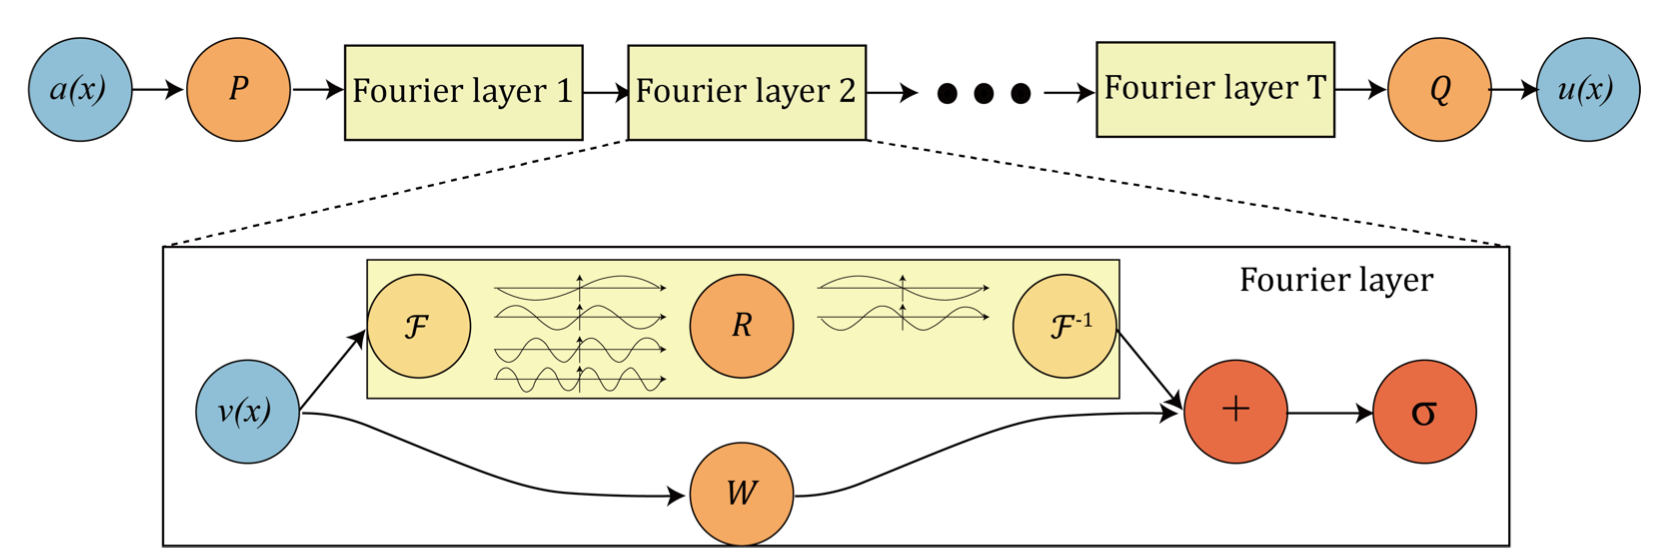
\includegraphics[width=0.99\textwidth]{architecture.png}
		\caption{Рис.  Структура нейронных Фурье операторов}
	\end{figure}

\subsection{Вычислительный эксперимент}
В работе Fourier Neural Operator for Parametric Partial Differential Equations были приведены эксперименты с нейронным Фурье оператором. Авторы работы сравнили предложенный ими нейронный Фурье оператор с несколькими конечномерными архитектурами на примере одномерного уравнения Бюргерса, двумерной задачи потока Дарси и двумерного уравнения Навье-Стокса.

Результаты представлены на рисунке 2.
\begin{figure}[h]
	\centering
	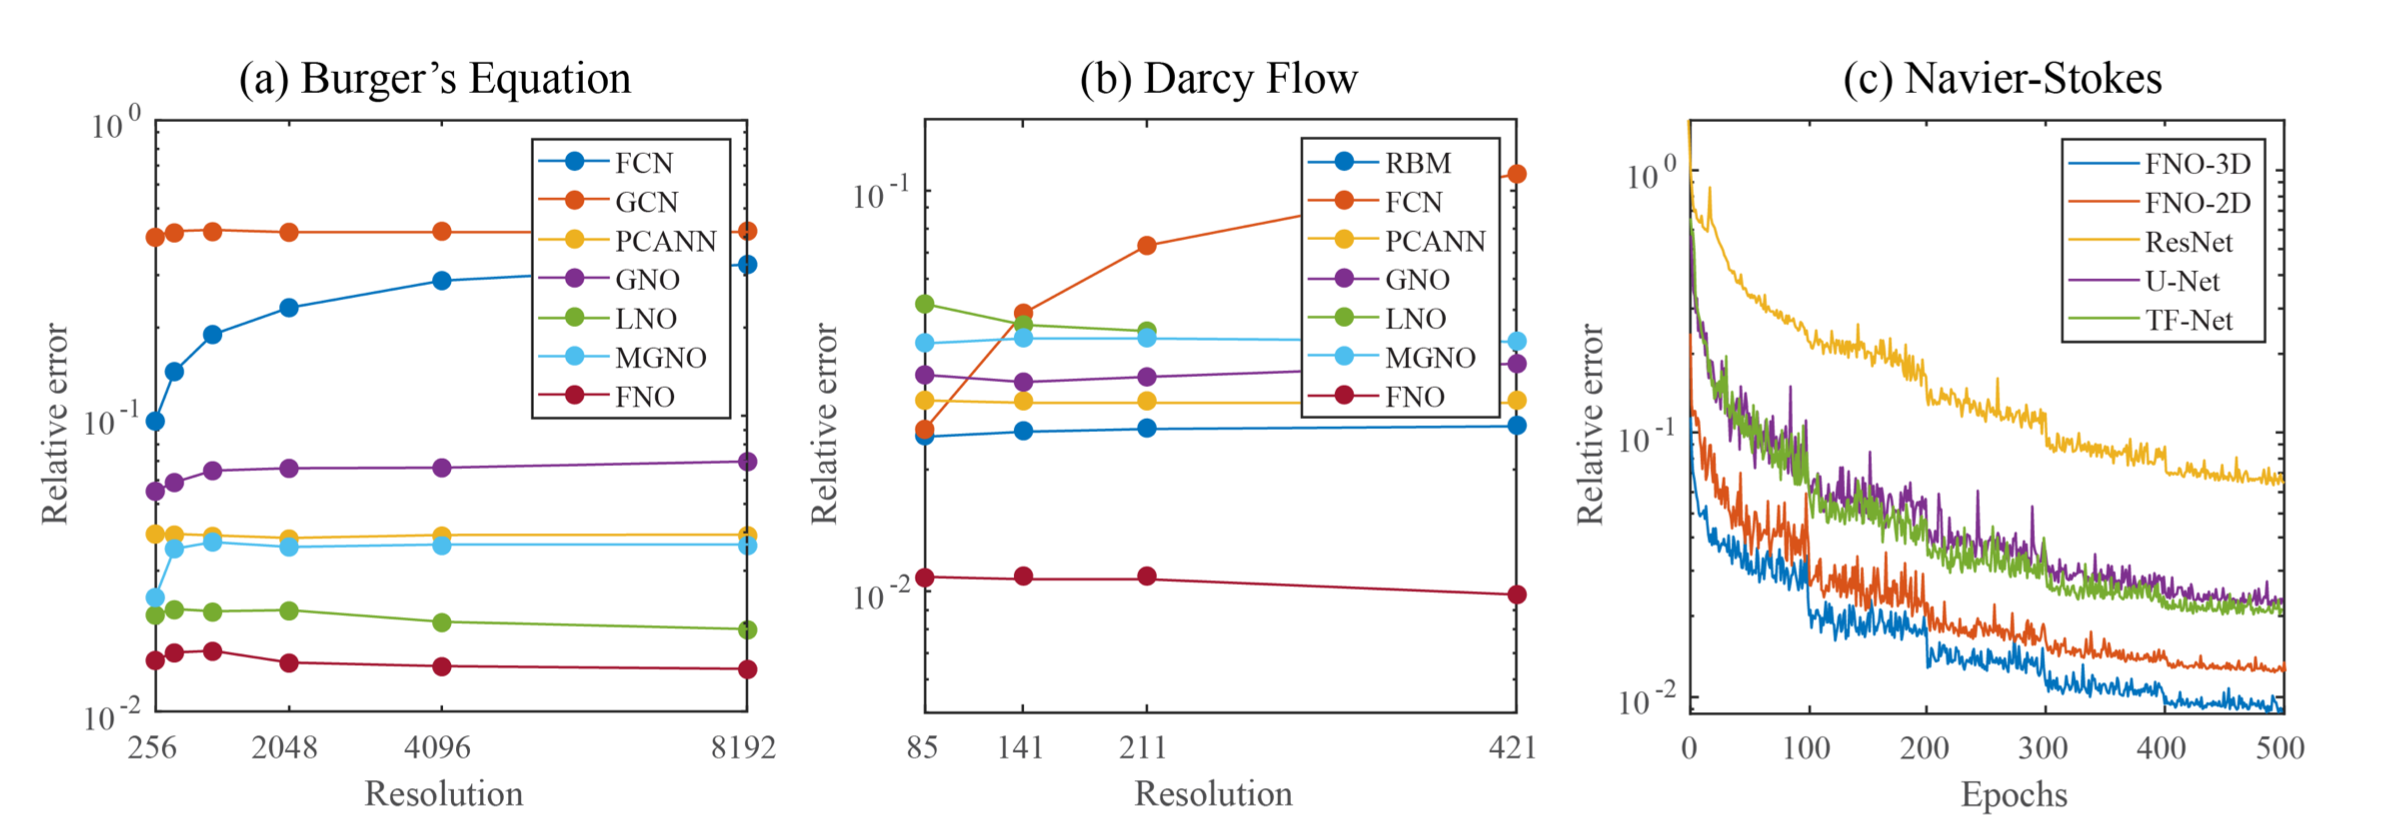
\includegraphics[width=0.99\textwidth]{experiments.png}
	\caption{Рис. Результаты экспериментов для уравнения Бюргерса, потоков Дарси, уравнениий Навье — Стокса}
\end{figure}

\begin{enumerate}
	\item \textbf{FNO}: the newly purposed Fourier neural operator.
	\item \textbf{FNO-2d}: 2-d Fourier neural operator with a RNN structure in time.
	\item \textbf{FNO-3d}: 3-d Fourier neural operator that directly convolves in space-time.
	\item NN: a simple point-wise feedforward neural network.
	\item RBM: the classical Reduced Basis Method (using a POD basis) 
	\item FCN: a the-state-of-the-art neural network architecture based on Fully Convolution Networks
	\item PCANN: an operator method using PCA as an autoencoder on both the input and output data and interpolating the latent spaces with a neural network
	\item GNO: the original graph neural operator
	\item MGNO: the multipole graph neural operator
	\item LNO: a neural operator method based on the low-rank decomposition of the kernel $\kappa(x, y):=\sum_{j=1}^{r} \phi_{j}(x) \psi_{j}(y)$ similar to the unstacked DeepONet
	\item ResNet: 18 layers of 2-d convolution with residual connections
	\item U-Net: A popular choice for image-to-image regression tasks consisting of four blocks with 2-d convolutions and deconvolutions
	\item TF-Net: A network designed for learning turbulent flows based on a combination of spatial and temporal convolutions 
	
\end{enumerate}


\subsection{Уравнения Навье-Стокса}
В работе также была приведена визуализация решения уравнений Навье-Стокса (Рис. 3)
$$
\begin{aligned}
\partial_{t} w(x, t)+u(x, t) \cdot \nabla w(x, t) &=\nu \Delta w(x, t)+f(x), & & x \in(0,1)^{2}, t \in(0, T] \\
\nabla \cdot u(x, t) &=0, & & x \in(0,1)^{2}, t \in[0, T] \\
w(x, 0) &=w_{0}(x), & & x \in(0,1)^{2}
\end{aligned}
$$

\begin{figure}[h]
	\centering
	%\includegraphics[width=1.02\textwidth]{experiment.pdf}
	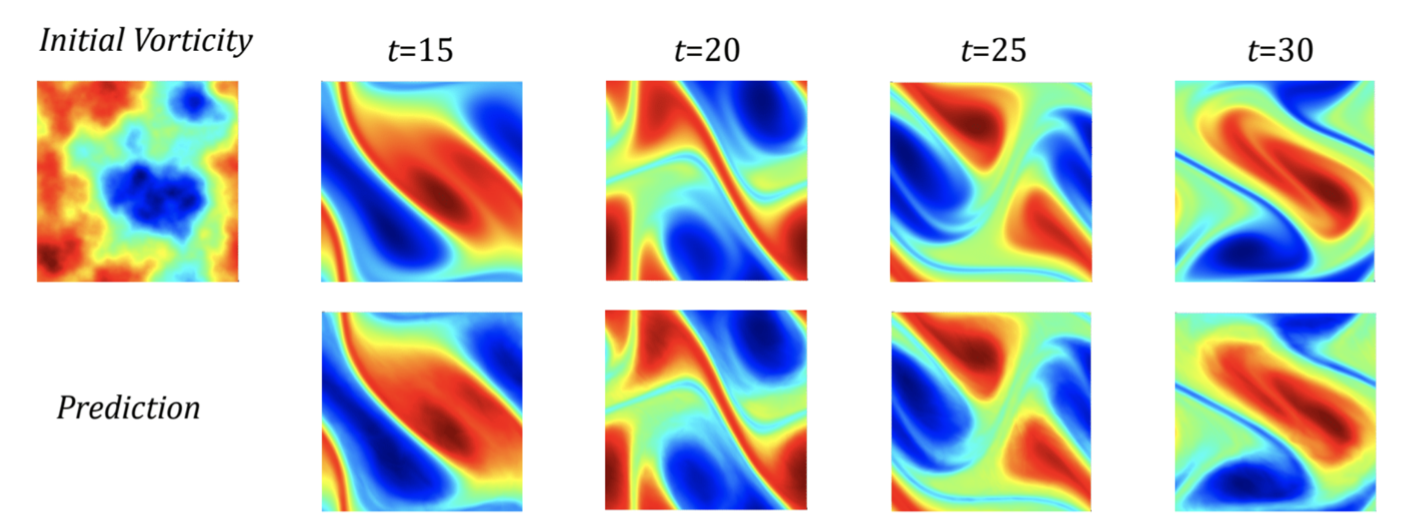
\includegraphics[width=0.99\textwidth]{navier_example.png}
	\caption{Рис. Пример потока из Навье-Стокса: истинные потоки сверху, предсказания нейронного Фурье оператора снизу}
	\label{fig:experiment}
\end{figure}

	
\section{Вопросы на обсуждение}

	\begin{itemize}
	\item Какие недостатки у традиционных методов решения по сравнения с нейронными Фурье  операторами?
	\item Как преобразование Фурье решает проблемы нейронного оператора? 
	\item Какие матрицы обучаются в слое нейронного Фурье оператора?
	\item Какая идея лежит в добавлении слагаемого $Wv_t(x)$ в слое нейронного оператора? 
\end{itemize}